\documentclass[11pt,a4paper]{article}
\usepackage[T1]{fontenc}
\usepackage{mathptmx}
\usepackage[margin=25mm]{geometry}
\usepackage{amsmath,amssymb}
\usepackage{graphicx}
\usepackage{booktabs,tabularx,array}
\usepackage[font=small,labelfont=bf]{caption}
\usepackage{placeins}
\usepackage{xurl}
\usepackage[hidelinks]{hyperref}
\graphicspath{{figures/}}
\linespread{1.04}
\setlength{\parskip}{0.12em}
\setlength{\tabcolsep}{5pt}
\renewcommand{\arraystretch}{1.15}
\hypersetup{pdftitle={Efficient Brain MRI Classification with Validation Guided Transfer Learning},pdfauthor={Vishesh Rao, Pranay Vishwakarma and Manu Vahan}}

\title{\textbf{Efficient Brain MRI Classification with\\Validation Guided Transfer Learning}}
\author{Vishesh Rao \and Pranay Vishwakarma \and Manu Vahan}
\date{\small Sajjan Agarwal School of Technology, Rishihood University\\Capstone Project Report\quad 3 November 2026}

\begin{document}
\maketitle

\begin{abstract}
This project reproduces a selected Xception baseline from Disci et al. (2025)
and investigates a smaller classifier for four-class brain MRI classification.
We use the pinned 7,023-image dataset and distinguish the original folder-based
protocol from an audited split that excludes known exact training--test overlap.
The selected baseline reproduction reaches 93.67\% clean test accuracy, compared
with the paper's 95.27\%. Under the audited protocol, the initial MobileNetV2
replacement fails the original performance-preservation hypothesis. Correcting
its ImageNet input normalization improves macro-F1 to 0.8062. We then compare a
longer-training control with a compact model combining Global Average Pooling,
frozen-backbone warm-up and low-rate fine-tuning with frozen BatchNorm statistics.
The compact model reaches 92.68\% test accuracy and 0.9256 macro-F1 with 2,422,468
parameters, 90.33\% fewer than the historical audited Xception reference
(0.9176 macro-F1). The final exploratory efficiency targets are met in this run.
Single-seed results, a previously examined test set and missing patient
identifiers limit generalization claims. Established techniques are evaluated;
no new algorithm or statistical superiority is claimed.
\end{abstract}
\noindent\textbf{Keywords:} brain MRI; tumor classification; transfer learning;
MobileNetV2; Xception; reproducibility.

\section{Introduction}
Brain MRI classification provides a practical setting for studying transfer
learning when labeled images and computational resources are limited. Our task
assigns individual MRI slices to glioma, meningioma, no tumor or pituitary tumor.
A useful capstone result should report predictive performance together with
model size and enough experimental evidence to reproduce the comparison.

Disci et al. evaluate six pretrained convolutional networks on a public MRI
collection and identify Xception as their best reported model~\cite{disci2025}.
We select that paper and its Xception model to establish one baseline. The scope is the selected Xception model. MobileNetV2 is our proposed
smaller replacement within this baseline-and-extension study.

Our work has three practical contributions. First, we implement and document
an approximate selected-model replication. Second, we audit exact image overlap
and preserve both favorable and unfavorable experiment outcomes. Third, we test
a compact classification head and validation-guided adaptation, with exported
checkpoints and a saved-model prediction demonstration. These contributions
concern experimental application and reproducibility, not algorithmic novelty.

\section{Selected Paper and Motivation}
The base paper uses transfer learning, preprocessing and augmentation on 7,023
images~\cite{disci2025}. Its Table~8 reports Xception test accuracy of 95.27\%
and macro-F1 of 0.9491. The headline 98.73\% weighted accuracy is consistent with
a sample-weighted combination of training and testing accuracy, as inferred
from its tables; we therefore use the Table~8 test score for comparison.

The paper identifies class-recall challenges, explainability, dataset diversity
and clinical validation as areas requiring further investigation. Our selected
extension examines the accuracy--parameter tradeoff and training stability.
MobileNetV2 uses inverted residuals and linear bottlenecks to support efficient
feature extraction~\cite{sandler2018}. Its architecture motivates testing a
smaller alternative, without assuming that its pretrained features will transfer
successfully to this MRI dataset.

The first smaller-model attempt leaves a substantial performance gap. This
motivates two questions: whether a longer validation-guided training policy
helps, and whether a smaller head with staged fine-tuning improves the tradeoff.
The warm-up and low-rate adaptation follow established transfer-learning
practice, including careful treatment of BatchNorm~\cite{kerasguide}.

\section{Dataset and Evaluation Protocols}
\subsection{Pinned dataset}
We use version~1 of Masoud Nickparvar's Brain Tumor MRI Dataset~\cite{dataset}.
It contains 7,023 images, matching the base paper. Version~2 contains 7,200
images and is excluded. Table~\ref{tab:data} gives the original folder counts.
The download URL, archive SHA256 and ordered image manifests are recorded.

\begin{table}[tb]
\centering
\caption{Original dataset version~1 folder counts.}
\label{tab:data}
\begin{tabular}{lrrrrr}
\toprule
Partition & Glioma & Meningioma & No tumor & Pituitary & Total\\
\midrule
Training & 1,321 & 1,339 & 1,595 & 1,457 & 5,712\\
Testing & 300 & 306 & 405 & 300 & 1,311\\
\bottomrule
\end{tabular}
\end{table}

\subsection{Overlap audit and splits}
Hashing decoded image pixels identifies 263 training images identical to test
images, 207 redundant images within training and 30 redundant images within
testing. No exact duplicate has conflicting labels. A perceptual-hash audit
also identifies 1,254 unresolved near-match candidate pairs; these are flagged
candidates, not verified patient matches.

We retain two distinct protocols. The \emph{paper-based} protocol keeps the
original folders and evaluates clean images and one fixed seeded transformed
test view, reflecting the source paper's test-augmentation description. The
\emph{audited} protocol removes exact training--test overlap and redundant
training copies, then reserves 15\% of the remaining training pool for
validation. It yields 4,518 training, 798 validation and 1,311 test images.
Training alone receives augmentation in the audited protocol.

Internal test duplicates remain. Reliable patient identifiers are unavailable,
so neither exact deduplication nor this split establishes patient independence.
All final experiments use the same ordered split fingerprint. Differences
between paper-based and audited results involve several protocol changes and
cannot isolate the effect of leakage removal.

\section{Methodology}
\subsection{Shared preprocessing}
Each slice is read in grayscale, smoothed with a Gaussian kernel of size~5,
thresholded at~45, and cropped to the bounding rectangle of the largest
foreground contour. The blurred grayscale crop is resized to $128\times128$,
replicated into three channels and scaled to $[0,1]$. The training pipeline
applies brightness and contrast factors in $[0.8,1.2]$. Foreground cropping
succeeds on all 7,023 images without a contour fallback. It is not a validated
tumor-segmentation procedure.

Kernel size, threshold, bounding-rectangle cropping, seed~42 and full backbone
trainability are disclosed implementation assumptions where the paper does not
provide a complete specification. These assumptions limit exact replication.
For normalization follow-ups, the model converts $[0,1]$ pixels to the documented
MobileNetV2 ImageNet range $[-1,1]$~\cite{mobilenetpreprocessing}. The operation
is saved inside the model, so inference does not normalize inputs twice.

\subsection{Baseline and original replacement}
The selected ImageNet backbone is followed by Flatten, Dropout(0.3), a
128-unit ReLU dense layer, Dropout(0.2), and a four-unit Softmax output.
The initial experiments fine-tune the complete backbone using Adam with
learning rate $10^{-4}$, batch size~20, sparse categorical cross-entropy and
five epochs. They evaluate the final-epoch checkpoint, preserving the
replication policy rather than selecting a checkpoint after viewing test scores.

The original hypothesis, H1, is that under identical audited settings,
MobileNetV2 will achieve macro-F1 no more than 0.02 below Xception while using
fewer total parameters. Both conditions are required. This original result
remains separate from all later exploratory experiments.

\subsection{Compact head and staged adaptation}
The final proposal replaces Flatten with Global Average Pooling (GAP).
For each channel $c$ of a feature tensor with height $H$, width $W$ and
$C$ channels, GAP computes
\begin{equation}
 g_c=\frac{1}{HW}\sum_{i=1}^{H}\sum_{j=1}^{W} F_{ijc},
 \qquad c=1,\ldots,C.
\end{equation}
Flatten preserves all $HWC$ entries; GAP produces $C$ values, reducing the
input size of the unchanged dense classifier. At our input resolution this
reduces the complete MobileNetV2 model from 4,880,068 to 2,422,468 parameters.
It does not provide a tumor mask or prove that the model attends to a lesion.

We define exploratory hypothesis H2 as improvement over normalized five-epoch
MobileNetV2 macro-F1 while using fewer parameters. The secondary target is a
macro-F1 gap of at most 0.02 from the saved audited Xception reference, also
with fewer parameters. Table~\ref{tab:methods} specifies the two new experiments.
Both start afresh from ImageNet weights and use identical audited data and
preprocessing.

\begin{table}[tb]
\centering\small
\caption{Predetermined control and proposed training policies.}
\label{tab:methods}
\begin{tabularx}{\linewidth}{@{}lXX@{}}
\toprule
Setting & A: training control & B: compact proposal\\
\midrule
Aggregation & Existing Flatten & Global Average Pooling\\
Total epoch budget & Up to 20 & 5 warm-up plus up to 15 fine-tuning\\
Warm-up & None & Backbone frozen; head rate $10^{-4}$\\
Fine-tuning & All layers at $10^{-4}$ & Non-BatchNorm layers at $10^{-5}$\\
BatchNorm statistics & Updated & Frozen throughout\\
Checkpoint & Minimum validation loss & Minimum validation loss across both stages\\
\bottomrule
\end{tabularx}
\end{table}

B completes five warm-up epochs, then begins fine-tuning from the final warm-up
weights. We recompile with a fresh Adam optimizer at the stage boundary.
BatchNorm layers remain frozen during fine-tuning. Head dropout remains active
during training. Fine-tuning stops after four consecutive epochs without lower
validation loss; its stopping counter resets at the stage boundary. The best
checkpoint is retained globally across both stages, including warm-up.

A tests a combined longer-budget and validation-selection policy. A versus B
tests a combined pooling, learning schedule and BatchNorm intervention. These
comparisons do not identify the individual causal effect of each component.

\section{Experimental Setup}
\subsection{Metrics and evidence}
For four classes, we report ordinary test accuracy and macro-F1,
\begin{equation}
 \operatorname{Accuracy}=\frac{N_{\mathrm{correct}}}{N},\qquad
 F_{1,\mathrm{macro}}=\frac14\sum_{c=1}^{4}
 \frac{2\mathrm{TP}_c}{2\mathrm{TP}_c+\mathrm{FP}_c+\mathrm{FN}_c}.
\end{equation}
Per-class recall, $\mathrm{TP}_c/(\mathrm{TP}_c+\mathrm{FN}_c)$, exposes uneven
errors. Weighted F1, balanced accuracy and ROC-AUC are retained in the machine-
readable evidence. Parameter reduction against reference $R$ is
$100(1-P/P_R)\%$, using total model parameters rather than trainable parameters.

We independently recompute metrics and confusion matrices from 1,311 ordered
saved predictions per experiment. Histories, manifests, configuration identity,
checkpoint SHA256 values and source-code matches are checked before accepting
the returned Colab runs. No new accuracy is inferred from a small demo sample.

\subsection{Runtime and checkpoint selection}
The new runs use the free Colab GPU workflow selected for a T4, Python~3.12.13,
TensorFlow~2.18.1, Keras~3.8.0, NumPy~2.0.2 and batch size~20. Recorded core
packages, platform and device descriptions match between A, B and the
normalization run. Historical Xception has a different recorded runtime
platform. Seed~42 and deterministic data ordering do not guarantee bitwise GPU
equivalence.

A completes 19 epochs, selects epoch~15 and has minimum validation loss 0.2617.
B completes 20 epochs, selects epoch~17 and has minimum validation loss 0.0937.
The lower validation loss also selects B for demonstration, independently of
test ranking. Test data never enters training or checkpoint-selection callbacks.
Because earlier experiments have already examined this test set, the final
comparison is exploratory rather than independent confirmatory validation.

\section{Results}
\subsection{Selected baseline reproduction}
Table~\ref{tab:replication} reports the paper-based baseline. Our clean Xception
accuracy is 1.60 percentage points below the published test accuracy. The
transformed view is 1.98 points below it. This is an approximate selected-model
replication, not an exact numerical reproduction of the entire paper.

\begin{table}[tb]
\centering
\caption{Paper-based Xception replication, separate from audited experiments.}
\label{tab:replication}
\begin{tabular}{lrr}
\toprule
Evaluation & Test accuracy (\%) & Macro-F1\\
\midrule
Published Table~8~\cite{disci2025} & 95.27 & 0.9491\\
Our clean test view & 93.67 & 0.9354\\
Our fixed transformed view & 93.29 & 0.9315\\
\bottomrule
\end{tabular}
\end{table}

\subsection{Original and normalization experiments}
Under the audited five-epoch protocol, original MobileNetV2 reaches 74.29\%
accuracy and 0.7372 macro-F1, compared with Xception's 91.76\% and 0.9176.
The 0.1804 macro-F1 gap exceeds the allowed 0.02 margin. H1 is therefore
unsupported despite an 80.52\% parameter reduction.

Changing only the configured input normalization improves MobileNetV2 to
81.92\% accuracy and 0.8062 macro-F1, an observed gain of 7.63 accuracy points
and 0.0690 macro-F1. Its 0.1114 gap to historical Xception still misses the
target. The earlier and normalized runs have different recorded runtime
platforms, so normalization is not established as the sole cause of the gain.

\subsection{Final performance and efficiency}
Table~\ref{tab:final} gives the complete audited progression. B improves on the
normalized five-epoch model by 10.76 accuracy points and 0.1194 macro-F1 while
using 50.36\% fewer parameters. Relative to A, B gains 3.97 accuracy points and
0.0415 macro-F1. H2's observed improvement-and-size criterion is met.

\begin{table}[tb]
\centering\small
\caption{Audited test results. Historical Xception uses different input scaling, training
budget and checkpoint policy; this is not a matched architecture comparison.}
\label{tab:final}
\begin{tabularx}{\linewidth}{@{}Xrrr@{}}
\toprule
Model or experiment & Accuracy (\%) & Macro-F1 & Parameters\\
\midrule
Historical Xception & 91.76 & 0.9176 & 25,056,428\\
Original MobileNetV2 & 74.29 & 0.7372 & 4,880,068\\
Normalized MobileNetV2 & 81.92 & 0.8062 & 4,880,068\\
A: longer-training control & 88.71 & 0.8841 & 4,880,068\\
\textbf{B: compact proposal} & \textbf{92.68} & \textbf{0.9256} & \textbf{2,422,468}\\
\bottomrule
\end{tabularx}
\end{table}

Relative to the saved audited Xception, B is 0.92 accuracy points and 0.0080
macro-F1 higher, with 90.33\% fewer parameters. Its observed gap satisfies the
secondary 0.02-margin target. This does not establish statistical superiority
or non-inferiority. B also uses a different protocol from the paper's published
95.27\% result; it must not be presented as outperforming that result.

Training takes 643.1 seconds (10.72 minutes) for A and 382.3 seconds (6.37
minutes) for B, including validation and checkpoint writes. Warmed batch-1
median inference times are 5.29 and 5.19 milliseconds, respectively, from 20
synchronized calls excluding image I/O and preprocessing. These are descriptive
single-run timings. Historical Xception trains for 239.2 seconds over five
epochs, so B does not train faster than that saved reference.

\begin{figure}[tb]
\centering
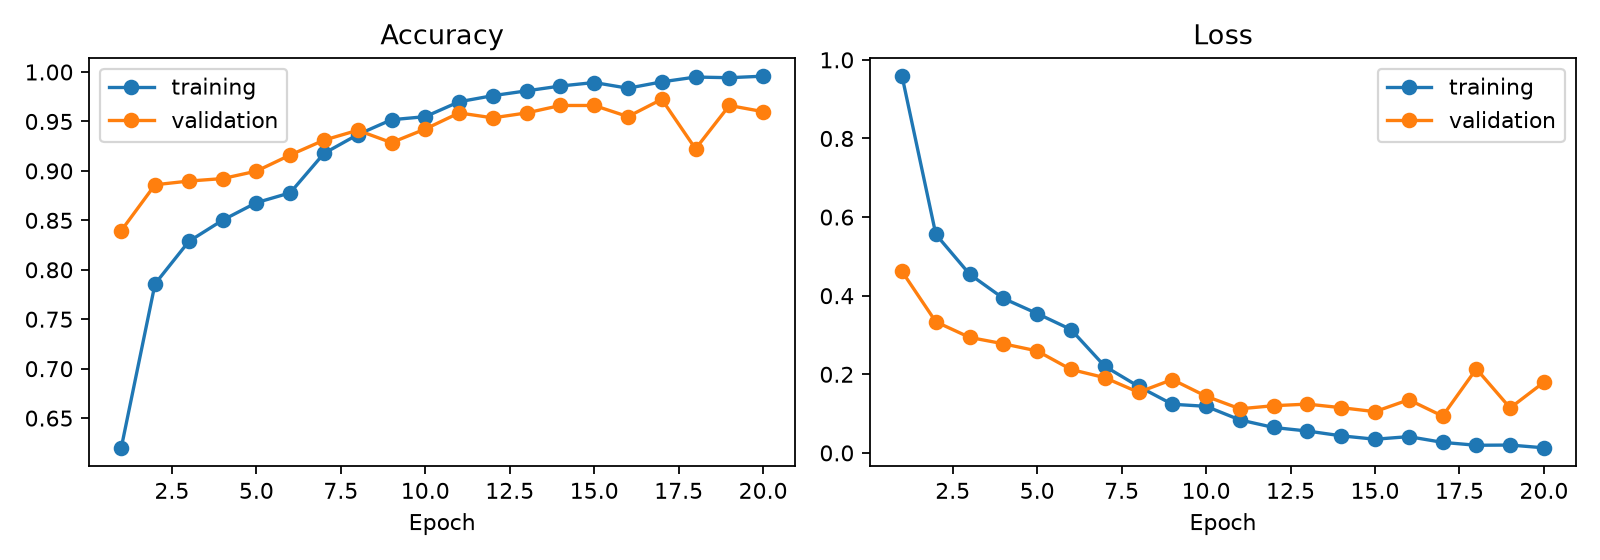
\includegraphics[width=\linewidth]{proposed_learning_curves.png}
\caption{Proposed model training and validation curves over 20 epochs. The
checkpoint is chosen by minimum validation loss at epoch~17, rather than the
final epoch or the test score. The first five epochs train the head only.}
\label{fig:curves}
\end{figure}

\subsection{Class-level error analysis}
Table~\ref{tab:recall} and Fig.~\ref{fig:confusion} show that improvement is not
uniform. Pituitary recall rises from 61.67\% in normalized five-epoch
MobileNetV2 to 97.67\% in B. However, B's meningioma and no-tumor recall are
slightly lower than A's. In particular, 38 of 306 meningioma slices are predicted
as no tumor, motivating further error analysis rather than an accuracy-only
conclusion.

\begin{table}[tb]
\centering
\caption{Class recall on the same audited test set.}
\label{tab:recall}
\begin{tabular}{lrr}
\toprule
Class & A recall (\%) & B recall (\%)\\
\midrule
Glioma & 91.00 & 93.67\\
Meningioma & 84.97 & 82.35\\
No tumor & 96.30 & 96.05\\
Pituitary & 80.00 & 97.67\\
\bottomrule
\end{tabular}
\end{table}

\begin{figure}[tb]
\centering
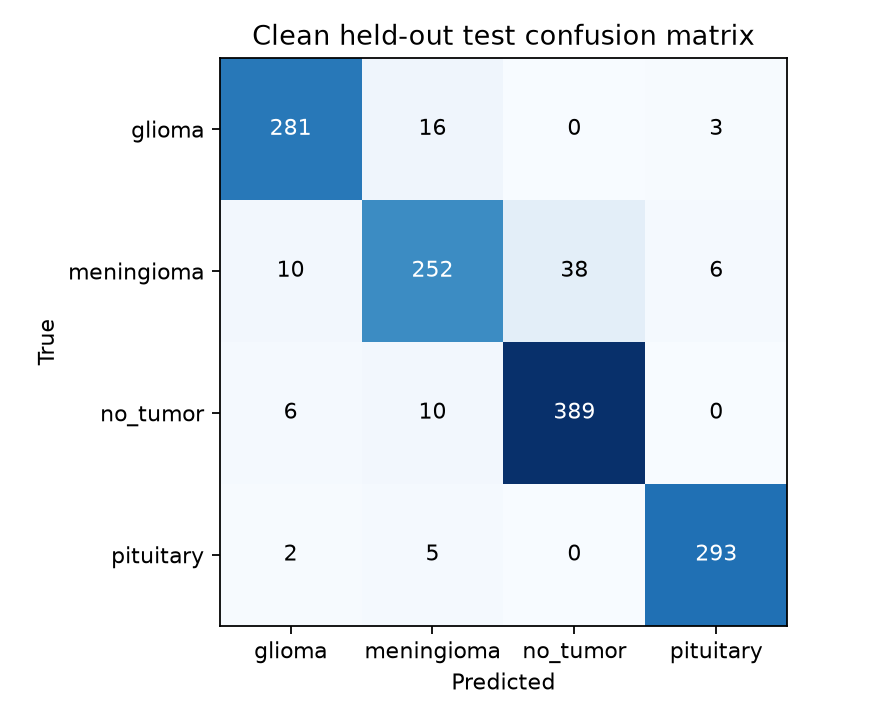
\includegraphics[width=0.64\linewidth]{proposed_confusion_matrix.png}
\caption{Proposed model confusion matrix from all 1,311 saved Colab test
predictions. Rows are dataset labels and columns are predictions.}
\label{fig:confusion}
\end{figure}
\FloatBarrier

\section{Saved Model Demonstration and Reproducibility}
Both accepted checkpoints load on the Mac CPU with the expected parameter
counts; all 52 BatchNorm layers are frozen in B's saved model. Four deterministic
first-per-class test images have verified decoded-pixel hashes. B predicts three
of four correctly, while A predicts two of four. All eight local predicted
classes agree with the corresponding saved Colab classes, including errors.
Maximum absolute CPU--GPU score differences are 0.0145 for B and 0.0538 for A;
their cause is unestablished. We do not claim strict probability equivalence or
separately reproduced full-test CPU accuracy.

Figure~\ref{fig:examples} uses the same clean glioma image shown in the Colab
demonstration and a recorded no-tumor error. The examples are the first test file
in each of these classes, not an estimate of class performance. Both examples have verified dataset provenance. Original images are shown
with their dataset and predicted labels; full-test prediction records provide
the quantitative evaluation.

\begin{figure}[tb]
\centering
\begin{minipage}[t]{0.46\linewidth}
\centering
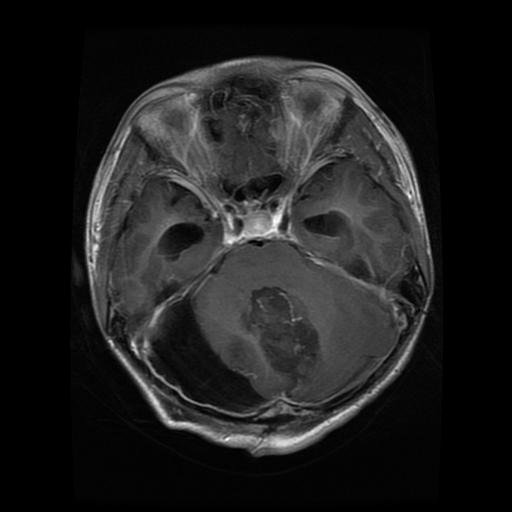
\includegraphics[width=0.82\linewidth]{example_glioma.jpg}\\[3pt]
\small (a) Dataset label: glioma\\Prediction: glioma
\end{minipage}\hfill
\begin{minipage}[t]{0.46\linewidth}
\centering
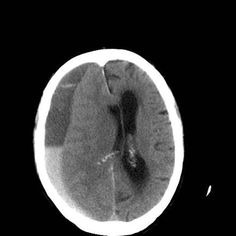
\includegraphics[width=0.82\linewidth]{example_no_tumor.jpg}\\[3pt]
\small (b) Dataset label: no tumor\\Prediction: meningioma
\end{minipage}
\caption{Correct and incorrect predictions from the proposed checkpoint,
consistent between the checked Mac CPU and saved Colab classes. Images are from
dataset version~1~\cite{dataset}. These examples do not establish diagnosis,
tumor localization or calibrated medical probabilities.}
\label{fig:examples}
\end{figure}

The repository contains the original executed Colab notebook, the baseline
reproduction notebook, the normalization notebook and the final training-extension
notebook. The latter displays verified saved results and model inference with
\texttt{RUN\_TRAINING=False}. The shared pipeline exposes simple \texttt{train},
\texttt{analyze} and \texttt{predict} commands. Forty-four automated tests cover
baseline behavior, staged training, checkpoint selection, BatchNorm handling,
evidence validation and resume checks. Synthetic test runs are not reported as
MRI research results. Full model exports are retained locally; weights and the
full raw dataset are excluded from Git.
\FloatBarrier

\section{Discussion and Limitations}
The final experiment provides a positive exploratory accuracy--size result and
an informative longer-training control. A's improvement demonstrates that the
initial five-epoch normalized model was not the strongest result obtainable
with that architecture and a validation-guided training policy. B further
improves macro-F1 with a smaller head and staged adaptation. Because the changes
are bundled, the result cannot isolate whether pooling, lower-rate adaptation,
BatchNorm handling or their interaction is responsible.

Several limitations remain. Only one seed is evaluated. Imaging modality and
clinical labels are taken from the supplied dataset and are not independently
verified. The test set has been
examined across project stages, so it is not an untouched confirmation set.
Exact overlap removal leaves unresolved perceptual near-matches and internal
test duplicates; missing patient identifiers prevent patient-level guarantees.
Historical Xception uses a different input-scaling convention, training budget,
selection policy and recorded runtime. Foreground cropping lacks segmentation annotations, and no
external clinical validation is performed. The observed margin is not a
statistical non-inferiority test. The method combines established components
rather than introducing a new learning algorithm.

Further work should repeat seeds, separately ablate pooling and fine-tuning
choices, inspect persistent meningioma errors, and obtain patient-level or
independent external validation. These steps would test the stability and scope
of the present finding.

\section{Conclusion}
We establish an approximate selected Xception replication and preserve an
initial unsupported smaller-model hypothesis. Normalization improves the first
MobileNetV2 result but does not preserve the target performance. A
subsequent compact, staged adaptation reaches 92.68\% accuracy and 0.9256
macro-F1, with 90.33\% fewer parameters than the saved audited Xception reference.
The final exploratory improvement and efficiency targets are met in this run.
The executed notebooks, checked prediction evidence, saved checkpoints and
reported errors support a reproducible demonstration while keeping the
remaining validation limits explicit.

\bibliographystyle{unsrt}
\bibliography{references}

\appendix
\section{Reproduction Information}
The code and notebooks are available at
\url{https://github.com/visheshrao17/ComputerVision_Prj/tree/feat/final-evaluation-normalization}.
The implementation and imported experiment evidence are recorded in commit
\texttt{bfbd165}. The LaTeX source, bibliography and figure assets accompany this
report and can be compiled in Overleaf with \texttt{main.tex} as the main document.
No GPU is required to read the stored notebook outputs.

The pinned dataset archive SHA256 is
\begin{center}\small\ttfamily
048b7413ce05bb52627046cfa5cde097b12e865aa80f6110959f547fd6fe4ef1
\end{center}
Experiment settings are in \path{configs/training_control.yaml} and
\path{configs/training_proposed.yaml}; compact evidence is under
\path{results/training_extension}. The reported split fingerprint is
\begin{center}\small\ttfamily
7d26f705e2895e05fbebdcb5487f2fa011ebc27ee71d2d04a2a93598d50af571
\end{center}
Both example images are illustrative report assets; the complete
raw dataset and model checkpoints are distributed separately from Git.

\end{document}
